% ============================================================================
% Manual de operación: simulación conjunta VaN3Twin (ns-3) + SUMO-GEO (visor 3D)
% Universidad de Cuenca — Redes Vehiculares y Heterogéneas (INGE-00104)
% Compilar: pdflatex -interaction=nonstopmode Manual_Simulacion_VaN3Twin_SUMO_GEO.tex (x2)
% Basado en MANUAL_SIMULACION_VAN3TWIN_SUMO_GEO.md (validado 25-ago-2026)
% ============================================================================
\documentclass[11pt,a4paper]{article}

\usepackage[utf8]{inputenc}
\usepackage[T1]{fontenc}
\usepackage{lmodern}
\usepackage{amssymb}
\usepackage[margin=2.2cm]{geometry}
\usepackage{xcolor}
\usepackage{graphicx}
\usepackage{booktabs}
\usepackage{enumitem}
\usepackage{fancyhdr}
\usepackage{tikz}
\usetikzlibrary{positioning,arrows.meta,shapes.geometric,calc}
\usepackage{listings}
\usepackage[most]{tcolorbox}
\usepackage{hyperref}

% ----------------------------------------------------------------------------
% Colores institucionales
% ----------------------------------------------------------------------------
\definecolor{azul}{HTML}{002856}
\definecolor{rojo}{HTML}{A51008}
\definecolor{gris}{HTML}{58585B}
\definecolor{verde}{HTML}{1A7A4A}
\definecolor{fondocodigo}{HTML}{F5F5F5}

\hypersetup{colorlinks=true, linkcolor=azul, urlcolor=rojo, citecolor=azul}

\pagestyle{fancy}
\fancyhf{}
\fancyhead[L]{\small\color{azul}\textbf{Manual VaN3Twin + SUMO-GEO}}
\fancyhead[R]{\small\color{gris}Redes Vehiculares y Heterogéneas}
\fancyfoot[C]{\small\thepage}
\renewcommand{\headrulewidth}{0.6pt}

% ----------------------------------------------------------------------------
% Listados de código
% ----------------------------------------------------------------------------
\lstdefinestyle{codigo}{
  backgroundcolor=\color{fondocodigo},
  basicstyle=\ttfamily\footnotesize,
  keywordstyle=\color{azul}\bfseries,
  commentstyle=\color{verde}\itshape,
  stringstyle=\color{rojo},
  numbers=none,
  breaklines=true,
  frame=single,
  rulecolor=\color{gris!40},
  framesep=4pt,
  showstringspaces=false,
  tabsize=2,
  columns=fullflexible,
  keepspaces=true
}
\lstset{style=codigo}

% ----------------------------------------------------------------------------
% Cajas "dónde se ejecuta cada paso"
% ----------------------------------------------------------------------------
\newtcolorbox{enmac}[1][]{
  colback=azul!4, colframe=azul, fonttitle=\bfseries, breakable,
  title={\faIconMac~EN EL MAC (PC local) #1}}
\newtcolorbox{encontenedor}[1][]{
  colback=rojo!4, colframe=rojo, fonttitle=\bfseries, breakable,
  title={\faIconDocker~DENTRO DEL CONTENEDOR \texttt{van3twin} #1}}
\newtcolorbox{ennavegador}[1][]{
  colback=verde!5, colframe=verde, fonttitle=\bfseries, breakable,
  title={\faIconEdit~EN EL NAVEGADOR #1}}
\newtcolorbox{notabox}[1][]{
  colback=gris!6, colframe=gris, fonttitle=\bfseries, breakable,
  title={Nota#1}}
\newtcolorbox{advertenciabox}{
  colback=rojo!6, colframe=rojo, fonttitle=\bfseries, breakable,
  title={Advertencia}}
\newtcolorbox{validadobox}{
  colback=verde!6, colframe=verde, fonttitle=\bfseries, breakable,
  title={Validado empíricamente (25-ago-2026)}}

% "iconos" simples (sin fuentes extra)
\newcommand{\faIconMac}{\tikz[baseline=-2pt]{\draw[azul,fill=azul!15,rounded corners=1pt] (0,0) rectangle (0.32,0.22); \draw[azul] (0.10,-0.05)--(0.22,-0.05);}}
\newcommand{\faIconDocker}{\tikz[baseline=-2pt]{\foreach \x in {0,0.11,0.22}{\draw[rojo,fill=rojo!15] (\x,0) rectangle (\x+0.09,0.09);}\foreach \x in {0.055,0.165}{\draw[rojo,fill=rojo!15] (\x,0.11) rectangle (\x+0.09,0.2);}}}
\newcommand{\faIconEdit}{\tikz[baseline=-2pt]{\draw[verde,fill=verde!15] (0,0) -- (0.22,0.22) -- (0.28,0.16) -- (0.06,-0.06) -- cycle;}}

\setlength{\parskip}{4pt}
\setlength{\parindent}{0pt}
\renewcommand{\contentsname}{Contenido}

% ============================================================================
\begin{document}

\begin{center}
  {\color{azul}\LARGE\bfseries Manual de operación}\\[4pt]
  {\color{azul}\Large\bfseries Simulación conjunta VaN3Twin + SUMO-GEO}\\[4pt]
  {\color{gris}\large Ejecutar una simulación V2X de ns-3 visualizada en 3D y en vivo en el navegador}\\[6pt]
  {\small Universidad de Cuenca --- Redes Vehiculares y Heterogéneas (INGE-00104)\\
  Prof.\ Pablo Barbecho --- 25 de agosto de 2026}
\end{center}

\vspace{2pt}
\hrule
\vspace{8pt}

\tableofcontents

% ============================================================================
\section{Qué hace esta integración}
% ============================================================================

VaN3Twin (framework V2X sobre ns-3) y SUMO-GEO (visor web 3D MapLibre/deck.gl)
se acoplan a la \textbf{misma} instancia de SUMO mediante TraCI
\emph{multi-cliente}: ns-3 es el cliente~1 (controla y marca el ritmo) y el
backend de SUMO-GEO es el cliente~2 (solo lectura). SUMO avanza en
\emph{lockstep} --- exige que ambos clientes pidan paso --- pero el visor pide
objetivos gruesos ($t+1$\,s), de modo que \textbf{no frena} a ns-3.

\begin{figure}[h!]
\centering
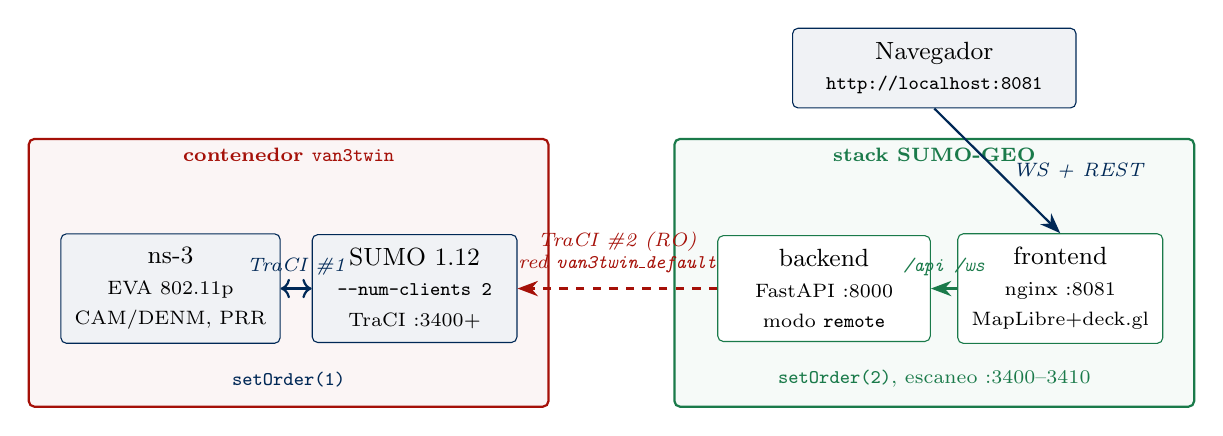
\begin{tikzpicture}[
  font=\small,
  caja/.style={draw, rounded corners=2pt, align=center, inner sep=5pt},
  flecha/.style={-{Stealth[length=2.6mm]}, thick},
  etiq/.style={font=\scriptsize\itshape, midway}
]
  \node[caja, draw=rojo, thick, fill=rojo!4, minimum width=6.6cm, minimum height=3.4cm] (van) at (-4.1,0) {};
  \node[anchor=north, font=\scriptsize\bfseries\color{rojo}] at (van.north) {contenedor \texttt{van3twin}};
  \node[caja, draw=azul, fill=azul!6, minimum width=2.6cm] (ns3) at (-5.6,-0.2)
        {ns-3\\\scriptsize EVA 802.11p\\\scriptsize CAM/DENM, PRR};
  \node[caja, draw=azul, fill=azul!6, minimum width=2.6cm] (sumo) at (-2.5,-0.2)
        {SUMO 1.12\\\scriptsize \texttt{--num-clients 2}\\\scriptsize TraCI :3400+};
  \draw[flecha, azul, <->] (ns3) -- (sumo) node[etiq, above=1pt] {TraCI \#1};
  \node[font=\scriptsize\color{azul}] at (-4.1,-1.35) {\texttt{setOrder(1)}};

  \node[caja, draw=verde, thick, fill=verde!4, minimum width=6.6cm, minimum height=3.4cm] (geo) at (4.1,0) {};
  \node[anchor=north, font=\scriptsize\bfseries\color{verde}] at (geo.north) {stack SUMO-GEO};
  \node[caja, draw=verde, fill=white, minimum width=2.7cm] (backend) at (2.7,-0.2)
        {backend\\\scriptsize FastAPI :8000\\\scriptsize modo \texttt{remote}};
  \node[caja, draw=verde, fill=white, minimum width=2.6cm] (nginx) at (5.7,-0.2)
        {frontend\\\scriptsize nginx :8081\\\scriptsize MapLibre+deck.gl};
  \draw[flecha, verde] (nginx) -- (backend) node[etiq, above=1pt] {\texttt{/api /ws}};
  \node[font=\scriptsize\color{verde}] at (4.1,-1.35) {\texttt{setOrder(2)}, escaneo :3400--3410};

  \draw[flecha, rojo, dashed, thick] (backend.west) -- (sumo.east)
        node[etiq, above=2pt, align=center] {TraCI \#2 (RO)\\red \texttt{van3twin\_default}};

  \node[caja, draw=azul, fill=azul!6, minimum width=3.6cm] (browser) at (4.1,2.6)
        {Navegador\\\scriptsize \texttt{http://localhost:8081}};
  \draw[flecha, azul, thick] (browser.south) -- (nginx.north)
        node[etiq, right=2pt] {WS + REST};
\end{tikzpicture}
\caption{Arquitectura validada: dos proyectos Docker Compose unidos por la red
\texttt{van3twin\_default}; la geometría del mapa se lee del volumen
\texttt{van3twin\_ns3-workspace}.}
\end{figure}

% ============================================================================
\section{Componentes, ubicaciones y puertos}
% ============================================================================

\begin{center}
\small
\begin{tabular}{@{}p{0.30\textwidth}p{0.32\textwidth}p{0.30\textwidth}@{}}
\toprule
\textbf{Pieza} & \textbf{Dónde} & \textbf{Rol} \\
\midrule
Stack van3twin & \texttt{\textasciitilde/van3twin-docker} & Contenedor \texttt{van3twin}: ns-3/VaN3Twin + SUMO 1.12.0 \\
Árbol ns-3 compilable & volumen Docker \texttt{van3twin\_ns3-workspace} & \textbf{Único} lugar donde se compila (case-sensitive) \\
Edición de código ns-3 & dentro del contenedor (\texttt{docker compose exec} o VS Code Dev Containers) & Se edita directamente en el volumen \\
Repo SUMO-GEO & \texttt{\textasciitilde/Dropbox/Mac/Documents/SUMO\_GEO} & Backend FastAPI + frontend MapLibre/deck.gl \\
Servicios del visor & profile \texttt{visor} del mismo \texttt{docker-compose.yml} de van3twin & backend (remote) + frontend nginx; solo arrancan con \texttt{-{}-profile visor} \\
\bottomrule
\end{tabular}
\end{center}

\begin{center}
\small
\begin{tabular}{@{}ll@{}}
\toprule
\textbf{Puerto (Mac)} & \textbf{Servicio} \\
\midrule
8081 & Visor SUMO-GEO (frontend nginx) \\
8000 & API del backend SUMO-GEO (\texttt{/api/health}, \texttt{/api/meta}\ldots) \\
8080 & vehicle-visualizer nativo de VaN3Twin (Leaflet 2D) \\
5901 & VNC del contenedor (GUI de SUMO) \\
8090 & GEO SUMO WEB de la práctica (percepción por radio) \\
3400+ & TraCI --- \textbf{no publicado}: solo red Docker interna \\
\bottomrule
\end{tabular}
\end{center}

% ============================================================================
\section{Requisitos previos (ya aplicados)}
% ============================================================================

El acoplamiento depende de estos parches, ya presentes y compilados. Verificar
solo si algo falla:

\begin{enumerate}[leftmargin=1.6em, itemsep=2pt]
  \item \textbf{\texttt{traci-client.cc}} (ns-3):
        \texttt{NS\_OBJECT\_ENSURE\_REGISTERED(TraciClient)} y llamada a
        \texttt{setOrder(1)} tras el \texttt{connect} cuando las opciones de
        SUMO contienen \texttt{-{}-num-clients}.
  \item \textbf{Ejemplo EVA} (\texttt{v2v-emergencyVehicleAlert-80211p.cc}):
        flag \texttt{-{}-num-traci-clients=N} que añade
        \texttt{-{}-num-clients N} al comando de SUMO.
  \item \textbf{Backend SUMO-GEO}: \texttt{sumo\_order}/\texttt{sumo\_port\_scan}
        en la configuración; \texttt{setOrder(2)} y escaneo de puertos
        3400--3410 al conectar; paso con objetivo absoluto; detección de
        proyección compatible con sumolib~1.12 (\texttt{geo.py}).
  \item \textbf{Servicios \texttt{backend}/\texttt{frontend}} (profile
        \texttt{visor} del compose de van3twin):
        \texttt{APP\_SUMO\_HOST=van3twin}, \texttt{APP\_SUMO\_PORT=3400},
        \texttt{APP\_SUMO\_PORT\_SCAN=10}, \texttt{APP\_SUMO\_ORDER=2}, y el
        net del EVA leído del volumen en solo lectura.
\end{enumerate}

\begin{enmac}[--- comprobación rápida]
\begin{lstlisting}[language=bash]
cd ~/van3twin-docker
docker compose exec van3twin grep -c "num-clients" src/traci/model/traci-client.cc   # >= 1
\end{lstlisting}
\end{enmac}

% ============================================================================
\section{Modos de ejecución y arranque}
% ============================================================================

Todo vive en un solo compose
(\texttt{\textasciitilde/van3twin-docker/docker-compose.yml}). Dos cosas
independientes definen el modo de operación: el \textbf{profile} decide qué
contenedores existen, y el flag \textbf{\texttt{-{}-num-traci-clients}}
decide, por corrida, si SUMO espera al visor. Van siempre en pareja
(figura~\ref{fig:modos}).

\begin{figure}[h!]
\centering
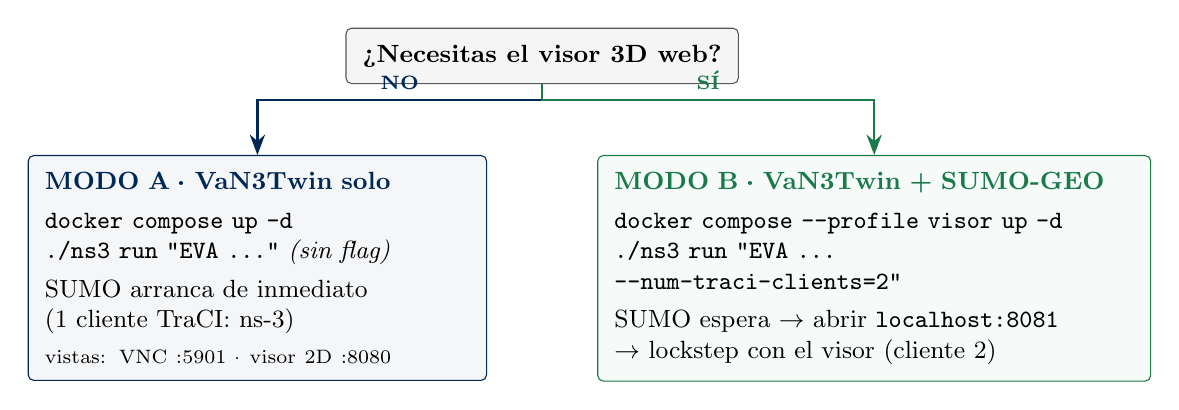
\begin{tikzpicture}[
  font=\small,
  caja/.style={draw, rounded corners=2pt, align=left, inner sep=6pt},
  flecha/.style={-{Stealth[length=2.6mm]}, thick},
  etiq/.style={font=\scriptsize\bfseries, midway}
]
  \node[caja, draw=gris, fill=gris!6, align=center] (q) at (0,0)
    {\textbf{¿Necesitas el visor 3D web?}};
  \node[caja, draw=azul, fill=azul!4, text width=5.4cm, below left=9mm and -18mm of q] (a)
    {\textbf{\color{azul}MODO A · VaN3Twin solo}\\[3pt]
     \texttt{docker compose up -d}\\
     \texttt{./ns3 run "EVA ..."} \emph{(sin flag)}\\[3pt]
     SUMO arranca de inmediato\\
     (1 cliente TraCI: ns-3)\\[2pt]
     \scriptsize vistas: VNC :5901 · visor 2D :8080};
  \node[caja, draw=verde, fill=verde!4, text width=6.6cm, below right=9mm and -18mm of q] (b)
    {\textbf{\color{verde}MODO B · VaN3Twin + SUMO-GEO}\\[3pt]
     \texttt{docker compose -{}-profile visor up -d}\\
     \texttt{./ns3 run "EVA ... -{}-num-traci-clients=2"}\\[3pt]
     SUMO espera $\rightarrow$ abrir \texttt{localhost:8081}\\
     $\rightarrow$ lockstep con el visor (cliente 2)};
  \draw[flecha, azul]  (q.south) -- ++(0,-2mm) -| node[etiq, above, pos=0.25]{NO} (a.north);
  \draw[flecha, verde] (q.south) -- ++(0,-2mm) -| node[etiq, above, pos=0.25]{SÍ} (b.north);
\end{tikzpicture}
\caption{Elección del modo de operación: el profile crea (o no) los
contenedores del visor; el flag hace que SUMO espere (o no) al segundo
cliente TraCI.}
\label{fig:modos}
\end{figure}

\begin{advertenciabox}
No levantar a la vez el \texttt{docker-compose.yml} normal del repo
\texttt{SUMO\_GEO} (modo \emph{managed}, para uso autónomo del visor):
comparte los puertos 8000/8081 con el Modo B y provocaría conflictos.
\end{advertenciabox}

\subsection*{Modo A --- VaN3Twin solo (uso clásico)}

\begin{center}
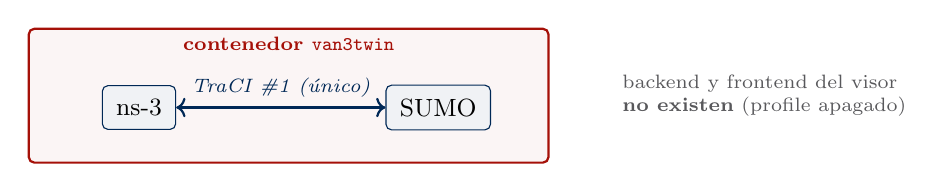
\begin{tikzpicture}[font=\small,
  caja/.style={draw, rounded corners=2pt, align=center, inner sep=5pt},
  flecha/.style={-{Stealth[length=2.4mm]}, thick}]
  \node[caja, draw=rojo, thick, fill=rojo!4, minimum width=6.6cm, minimum height=1.7cm] (van) at (0,0) {};
  \node[anchor=north, font=\scriptsize\bfseries\color{rojo}] at (van.north) {contenedor \texttt{van3twin}};
  \node[caja, draw=azul, fill=azul!6] (ns3) at (-1.9,-0.15) {ns-3};
  \node[caja, draw=azul, fill=azul!6] (sumo) at (1.9,-0.15) {SUMO};
  \draw[flecha, azul, <->] (ns3) -- node[font=\scriptsize\itshape, above]{TraCI \#1 (único)} (sumo);
  \node[align=left, font=\scriptsize\color{gris}, right=8mm of van]
    {backend y frontend del visor\\\textbf{no existen} (profile apagado)};
\end{tikzpicture}
\end{center}

\begin{enmac}
\begin{lstlisting}[language=bash]
cd ~/van3twin-docker && docker compose up -d   # sin --profile: el visor no arranca
docker compose exec van3twin bash
\end{lstlisting}
\end{enmac}

\begin{encontenedor}
\begin{lstlisting}[language=bash]
./ns3 run "v2v-emergencyVehicleAlert-80211p --sumo-gui=false --met-sup=true"
\end{lstlisting}
\end{encontenedor}

\textbf{Sin} \texttt{-{}-num-traci-clients}: SUMO no espera a nadie y la
simulación arranca de inmediato. Opcionales: GUI de SUMO por VNC
(\texttt{open vnc://127.0.0.1:5901} en el Mac y quitar
\texttt{-{}-sumo-gui=false}) o el visor 2D nativo
(\texttt{-{}-vehicle-visualizer=true} $\rightarrow$ \texttt{:8080}).

\subsection*{Modo B --- VaN3Twin + visor 3D SUMO-GEO (profile \texttt{visor})}

\begin{center}
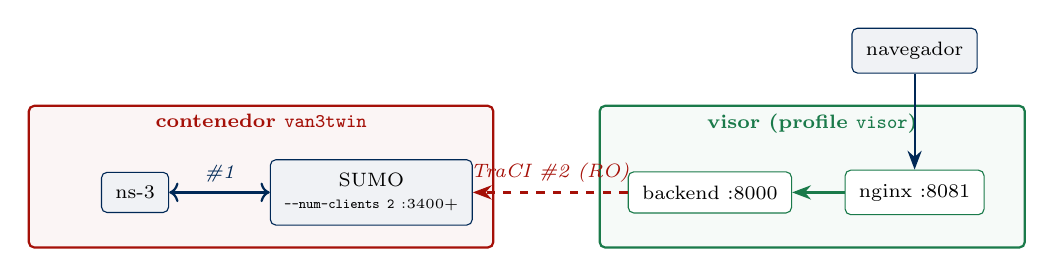
\begin{tikzpicture}[font=\small,
  caja/.style={draw, rounded corners=2pt, align=center, inner sep=5pt},
  flecha/.style={-{Stealth[length=2.4mm]}, thick},
  etiq/.style={font=\scriptsize\itshape, midway}]
  \node[caja, draw=rojo, thick, fill=rojo!4, minimum width=5.9cm, minimum height=1.8cm] (van) at (-3.4,0) {};
  \node[anchor=north, font=\scriptsize\bfseries\color{rojo}] at (van.north) {contenedor \texttt{van3twin}};
  \node[caja, draw=azul, fill=azul!6, font=\scriptsize] (ns3) at (-5.0,-0.2) {ns-3};
  \node[caja, draw=azul, fill=azul!6, font=\scriptsize, align=center] (sumo) at (-2.0,-0.2)
    {SUMO\\\tiny\texttt{--num-clients 2} :3400+};
  \draw[flecha, azul, <->] (ns3) -- node[etiq, above]{\#1} (sumo);
  \node[caja, draw=verde, thick, fill=verde!4, minimum width=5.4cm, minimum height=1.8cm] (geo) at (3.6,0) {};
  \node[anchor=north, font=\scriptsize\bfseries\color{verde}] at (geo.north) {visor (profile \texttt{visor})};
  \node[caja, draw=verde, fill=white, font=\scriptsize] (backend) at (2.3,-0.2) {backend :8000};
  \node[caja, draw=verde, fill=white, font=\scriptsize] (nginx) at (4.9,-0.2) {nginx :8081};
  \draw[flecha, verde] (nginx) -- (backend);
  \draw[flecha, rojo, dashed, thick] (backend.west) -- node[etiq, above]{TraCI \#2 (RO)} (sumo.east);
  \node[caja, draw=azul, fill=azul!6, font=\scriptsize] (br) at (4.9,1.6) {navegador};
  \draw[flecha, azul] (br) -- (nginx);
\end{tikzpicture}
\end{center}

\begin{enmac}
\begin{lstlisting}[language=bash]
cd ~/van3twin-docker && docker compose --profile visor up -d
\end{lstlisting}
\end{enmac}

y seguir la \S\ref{sec:ejecutar} (Pasos A--B--C) lanzando el EVA \textbf{con}
\texttt{-{}-num-traci-clients=2}. Flag y visor van siempre juntos: con el flag
SUMO espera al visor; sin el flag, el visor no puede conectar (pantalla en
negro).

\begin{notabox}
Se puede alternar entre modos sin tocar contenedores: si el visor ya está
arriba pero se lanza sin el flag, la simulación corre sola (Modo A) y el visor
simplemente no conecta en esa corrida.
\end{notabox}

\subsection*{Mantenimiento del stack}

\begin{notabox}[: cuándo usar \texttt{-{}-build}]
\texttt{docker compose -{}-profile visor build backend} $+$ \texttt{up -d} solo si
cambió algo de \texttt{backend/} del repo \texttt{SUMO\_GEO} (código Python,
requirements o Dockerfile). Uso diario $\Rightarrow$ nada: el stack queda
corriendo en segundo plano.
\end{notabox}

% ============================================================================
\section{Ejecutar una simulación con el visor (el orden importa)}
\label{sec:ejecutar}
% ============================================================================

\subsection*{Paso A --- limpiar restos de la corrida anterior}

\begin{encontenedor}
\begin{lstlisting}[language=bash]
cd ~/van3twin-docker && docker compose exec van3twin bash
# dentro del contenedor:
pkill -f ns3-dev-v2v; pkill sumo; sleep 1      # inofensivo si no hay nada
\end{lstlisting}
\end{encontenedor}

\subsection*{Paso B --- lanzar el EVA pidiendo 2 clientes TraCI}

\begin{encontenedor}
\begin{lstlisting}[language=bash]
./ns3 run "v2v-emergencyVehicleAlert-80211p --sumo-gui=false --met-sup=true --num-traci-clients=2"
\end{lstlisting}
\end{encontenedor}

Salida esperada:

\begin{lstlisting}
***Starting server on port 34XX ***
  waiting for 2 clients...
  client connected
\end{lstlisting}

\ldots{}y ahí \textbf{se queda esperando}. Es el comportamiento correcto: SUMO
no arranca hasta que conecte el visor (cliente 2).

\begin{notabox}[: el puerto puede variar]
El puerto puede ser 3400, 3401, 3402\ldots{}: el cliente TraCI de ns-3
(\texttt{GetFreePort}) salta al siguiente puerto libre si el anterior quedó en
estado TCP \texttt{TIME\_WAIT} ($\approx$60\,s tras cada corrida). El backend
escanea 3400--3410 y lo encuentra solo; no hay que configurar nada.
\end{notabox}

\subsection*{Paso C --- abrir (o recargar) el visor}

\begin{ennavegador}
Abrir \url{http://localhost:8081}. Al conectar el WebSocket, en el terminal
aparece el segundo \texttt{client connected} seguido de
\texttt{Simulation version 1.12.0 started}: todo corre en lockstep. El visor
abre sobre \textbf{Turín} con los 7--8 vehículos del EVA.
\end{ennavegador}

\begin{validadobox}
Secuencia completa observada en producción: \texttt{waiting for 2 clients}
$\rightarrow$ conectan ns-3 (orden 1) y el backend (orden 2) $\rightarrow$
lockstep sin frenar a ns-3 $\rightarrow$ visor 3D en vivo;
\texttt{/api/health} responde
\texttt{\{"status":"ok","mode":"remote"\}}.
\end{validadobox}

\subsection*{Reglas de la sesión}

\begin{itemize}[leftmargin=1.6em, itemsep=2pt]
  \item \textbf{Un visor por corrida.} No recargar la página a mitad de
        simulación ni abrir una segunda pestaña: SUMO fijó 2 clientes al
        arrancar. Tras una recarga, volver al Paso~A.
  \item No usar el selector Bajo/Medio/Alto del visor (pertenece al modo
        \emph{managed}).
  \item Al terminar (\texttt{-{}-sim-time} o fin de rutas), VaN3Twin cierra
        SUMO (\texttt{-{}-quit-on-end}) y el visor pierde la conexión: es lo
        esperado. ns-3 imprime su resumen (CAMs, PRR, etc.).
  \item Nueva corrida $=$ Paso~A $\rightarrow$ B $\rightarrow$ C. El stack
        SUMO-GEO sigue arriba; no se toca.
\end{itemize}

% ============================================================================
\section{Flags útiles del ejemplo EVA}
% ============================================================================

\begin{center}
\small
\begin{tabular}{@{}p{0.38\textwidth}p{0.54\textwidth}@{}}
\toprule
\textbf{Flag} & \textbf{Efecto} \\
\midrule
\texttt{-{}-num-traci-clients=2} & \textbf{Obligatorio para el visor}: SUMO espera 2 clientes TraCI \\
\texttt{-{}-sim-time=250} & Duración de la simulación (s) \\
\texttt{-{}-csv-log=nombre} & Log CSV por vehículo de la aplicación EVA \\
\texttt{-{}-sumo-updates=0.1} & Sincronización TraCI cada 0.1\,s sim (default 0.01) $\rightarrow$ $\sim$10$\times$ menos overhead, acelera el lockstep \\
\texttt{-{}-met-sup=true} & Metric supervisor (PRR, latencia) \\
\texttt{-{}-vehicle-visualizer=true} & Visor 2D nativo además del 3D (\texttt{:8080}) \\
\texttt{-{}-send-cam=false} & Desactiva la transmisión de CAMs (escenario de referencia) \\
\texttt{-{}-penetrationRate=0.5} & Fracción de vehículos con equipo V2X \\
\bottomrule
\end{tabular}
\end{center}

\begin{advertenciabox}
Sin espacios dentro de cada flag: el \texttt{./ns3 run} de este fork parte la
cadena por espacios \emph{sin respetar comillas internas}.
\end{advertenciabox}

% ============================================================================
\section{Velocidad de la simulación en el visor}
% ============================================================================

El slider \textbf{Velocidad (fps)} de la web sí actúa: cada movimiento envía
\texttt{\{cmd:"speed"\}} al backend, que pide a SUMO un avance de
\texttt{APP\_STEP\_LENGTH} (1\,s simulado) por frame. El techo del visor es por
tanto $\text{fps}\times 1$\,s: a 10\,fps hasta 10$\times$ tiempo real, a
30\,fps hasta 30$\times$. Pero en \emph{lockstep} manda el cliente más lento,
y suele ser \textbf{ns-3}: el EVA sincroniza TraCI cada
\texttt{sumo\_updates}\,$=0{,}01$\,s simulados por defecto
($\sim$100 sincronizaciones por segundo de simulación).

Para acelerar, en este orden:

\begin{enumerate}[leftmargin=1.6em, itemsep=2pt]
  \item \texttt{-{}-sumo-updates=0.1} en el comando del EVA (mayor impacto:
        $\sim$10$\times$ menos sincronizaciones TraCI; posiciones cada
        0.1\,s sim, de sobra para el visor).
  \item Subir el slider a 20--30\,fps.
  \item \texttt{APP\_STEP\_LENGTH} mayor (2--5) en el compose de integración:
        más rápido, pero el movimiento se ve a saltos.
  \item Quitar carga a ns-3 si no se necesita en esa corrida:
        \texttt{-{}-met-sup=false}, sin \texttt{-{}-csv-log}.
\end{enumerate}

\begin{notabox}[: fluidez (25-ago)]
El frontend \textbf{interpola el movimiento entre frames} (posición y rumbo,
con detección de teletransportes) y el default pasó a
\texttt{APP\_STEP\_LENGTH=0.5}. La interpolación refresca \textbf{solo la capa
de vehículos} y adapta su ritmo a la flota (60\,fps hasta 150 vehículos
$\rightarrow$ $\sim$11\,fps hasta 1500; por encima se desactiva).
\end{notabox}

\begin{advertenciabox}
\textbf{Con flotas grandes hay dos límites distintos.} (1)~\emph{Render
(frontend)}: resuelto con lo anterior. (2)~\emph{ns-3 (VaN3Twin)}: el coste
por segundo simulado crece con el número de nodos (CAM/CPM broadcast
$\approx O(N^2)$ recepciones) y \textbf{ns-3 es mono-hilo} --- más CPUs de
Docker no lo aceleran. Si ns-3 no da abasto, los frames del visor llegan
tarde; la interpolación mide el intervalo real y estira el movimiento
(fluido, pero más lento que tiempo real). Palancas:
\texttt{-{}-sumo-updates=0.1}, \texttt{-{}-penetrationRate=0.5} (menos nodos
radio sin quitar vehículos de SUMO), \texttt{-{}-met-sup=false}, sin
\texttt{-{}-csv-log}. Guía de \texttt{APP\_STEP\_LENGTH}: flotas pequeñas
($<$50) $\rightarrow$ 0.2--0.5; flotas grandes $\rightarrow$
\textbf{0.5--1.0} (menos frames y menos payload por segundo simulado; la
interpolación aporta la suavidad).
\end{advertenciabox}

% ============================================================================
\section{Qué ofrece el visor durante la corrida}
% ============================================================================

Vehículos 3D procedurales a su tamaño y rumbo reales; calles coloreadas por
nivel de servicio (LOS A--F) según la densidad en vivo; semáforos
sincronizados con las fases de SUMO; \textbf{clic derecho} sobre un
vehículo, calle o semáforo abre el inspector (velocidad, CO$_2$, combustible,
ruido, tiempo perdido, carril, progreso de ruta\ldots); panel de
\emph{Históricos} con series en vivo (vehículos por tipo, CO$_2$ de flota,
tiempo de viaje, esperas en semáforo); capa de calles concurridas; presets de
iluminación (amanecer/día/atardecer/noche) y cámara 2D/3D con auto-órbita.

\begin{notabox}
El visor muestra la \emph{verdad terreno} de SUMO (todos los vehículos). La
\emph{percepción por radio} (CAMs recibidos por cada nodo) se analiza con los
\texttt{.pcap}/CSV de ns-3 (Wireshark: filtros \texttt{gnw}, \texttt{btpb},
\texttt{its}) o con el GEO SUMO WEB de la práctica (\texttt{:8090}).
Son vistas complementarias.
\end{notabox}

% ============================================================================
\section{Editar código y recompilar}
\label{sec:editar}
% ============================================================================

El árbol vive en el volumen \texttt{van3twin\_ns3-workspace} y \textbf{se
edita directamente ahí}, dentro del contenedor
(\texttt{docker compose exec van3twin bash} + nano/vim, o VS Code con la
extensión \emph{Dev Containers} adjuntada al contenedor \texttt{van3twin};
ruta \texttt{/home/vanet/VaN3Twin/ns-3-dev}).

\textbf{Después de editar, según el tipo de fichero:}

\begin{center}
\small
\begin{tabular}{@{}p{0.38\textwidth}p{0.54\textwidth}@{}}
\toprule
\textbf{Qué editaste} & \textbf{Qué hacer después} \\
\midrule
C++ (\texttt{src/**/*.cc}, \texttt{*.h}) & \texttt{./ns3 build} (incremental) $\rightarrow$ relanzar la simulación (Pasos A--B--C) \\
\texttt{CMakeLists.txt} o ejemplo nuevo & \texttt{./ns3 build} (re-ejecuta cmake solo) $\rightarrow$ relanzar \\
Escenario SUMO (\texttt{.rou.xml}, \texttt{.sumocfg}, \texttt{.net.xml}) & Nada que compilar: relanzar la simulación. Si cambió el \textbf{net}, también \texttt{up -d} del stack SUMO-GEO (el backend carga la geometría al arrancar) \\
Backend SUMO-GEO (Mac, \texttt{backend/}) & \texttt{docker compose -{}-profile visor build backend} $+$ \texttt{up -d} (desde \texttt{\textasciitilde/van3twin-docker}) \\
Frontend SUMO-GEO (Mac, \texttt{frontend/}) & Nada: recargar el navegador (nginx lo sirve montado). Si el cambio no aparece: \textbf{recarga dura \textsf{Cmd+Shift+R}} (descarta el \texttt{app.js} cacheado) \\
\bottomrule
\end{tabular}
\end{center}

\begin{advertenciabox}
\textbf{Copia de seguridad:} las ediciones viven \emph{solo} en el volumen ---
\texttt{docker compose down -v} las borra. Para versionar, el árbol tiene git
dentro (\texttt{cd \textasciitilde/VaN3Twin/ns-3-dev \&\& git add -A
src/automotive src/traci \&\& git commit}); o exporta ficheros puntuales a
\texttt{\textasciitilde/results} (visible en el Mac). \textbf{Nunca} montar el
árbol como bind mount del Mac ni compilar desde una carpeta APFS: los pares de
ficheros que solo difieren en mayúsculas (\texttt{ActionID/ActionId},
\texttt{BOOLEAN/boolean}\ldots) colisionan y rompen la compilación.
\end{advertenciabox}

% ============================================================================
\section{Replay offline: mensajes V2X desde los .pcap}
% ============================================================================

Reproduce una corrida \textbf{grabada} en el visor 3D con el intercambio de
mensajes real: pulso radial en cada transmisión, arco TX$\rightarrow$RX por
cada recepción (color por tipo: CAM azul, CPM verde, DENM rojo) y, con
\textbf{clic izquierdo sobre un pulso}, el \textbf{contenido ASN.1 completo}
del mensaje más la lista de receptores. No necesita SUMO ni TraCI: la
movilidad se reconstruye de los encabezados GeoNetworking y los mensajes se
decodifican con los \texttt{.asn} oficiales ETSI del árbol de VaN3Twin.

\begin{encontenedor}[--- tras la corrida]
\begin{lstlisting}[language=bash]
cp ~/VaN3Twin/ns-3-dev/v2v-EVA-*.pcap ~/results/
\end{lstlisting}
\end{encontenedor}

\begin{enmac}
\begin{lstlisting}[language=bash]
# nada mas que hacer: el backend detecta los ficheros nuevos de ~/results
# automaticamente (al pulsar Replay o al consultar la API) y recarga el indice
curl localhost:8000/api/replay/info   # totales por tipo y PDR por par
\end{lstlisting}
\end{enmac}

\begin{ennavegador}
Los controles viven en el panel \textbf{Replay V2X} (columna izquierda,
debajo del panel SUMO·GEO): botón \emph{Replay pcap}, línea de tiempo con
\emph{seek}, botón play/pausa, y botones
$\blacktriangleleft$/$\blacktriangleright$ (paso atrás/adelante: salta un frame y pausa, con los mensajes congelados en
pantalla; clic sobre cualquier \textbf{pulso o arco} abre la
\textbf{disección por capas} estilo Wireshark --- 802.11 $\rightarrow$
GeoNetworking $\rightarrow$ BTP-B $\rightarrow$ ITS/ASN.1, secciones
plegables con scroll), selector de vehículo emisor (All/vehX; al elegir uno, el vehículo se resalta con un anillo ámbar en el mapa) y filtros
CAM/CPM/DENM. Debajo, el panel \textbf{PHY 802.11p} con las métricas de capa
física de la corrida: banda/canal/BW/modulación y potencia TX (config.\ del
EVA), latencia TX$\rightarrow$RX medida (media/p95/máx), rango de cobertura
observado, PER global (RX logradas vs.\ esperadas según coexistencia), PDR
mejor/peor par, tasas por tipo y utilización de canal estimada por airtime. Los \textbf{enlaces llevan etiqueta con la distancia en
metros} (visible en paso/pausa o con pocos arcos) y el popup lista cada
receptor con su distancia. La potencia RX no viene en los pcap (sin
radiotap), pero un \texttt{signal-rx.csv} en \texttt{\textasciitilde/results}
(callbacks SignalInfo del EVA; formato \texttt{rx,tx,t\_ms,rssi[,snr]};
código en \texttt{Practica\_Replay\_V2X.pdf}) se ingiere solo y añade el RSSI
a etiquetas, popup y panel PHY. Los paneles se auto-ocultan a su barra de título; el pin del
título los fija.
\end{ennavegador}

\begin{notabox}
El uso didáctico completo --- incluido el análisis de los mismos pcaps con
Wireshark y el contraste entre ambas vistas --- está en la práctica aparte:
\texttt{Practica\_Replay\_V2X.pdf}.
\end{notabox}

\begin{notabox}[: notas técnicas]
Movilidad desde la posición del emisor en cada paquete ($\sim$10\,Hz;
vehículos que nunca transmiten no aparecen). El pool de nodos de ns-3 se
reutiliza entre vehículos: el replay lo resuelve por segmentos temporales
decodificando los CAM. Arcos RX muestreados a $\leq$400 por frame. GN Beacons
excluidos. Decodificación validada (SUMO 1.12 + VaN3Twin ago-2026): CAM
(EN\,302\,637-2), CPM~v2 (\texttt{CPM-all.asn} --- no usar la variante
TR\,103\,562+ISO\,19091: tarda minutos en compilar), DENM.
\end{notabox}

% ============================================================================
\section{Solución de problemas}
% ============================================================================

\begin{center}
\small
\begin{tabular}{@{}p{0.30\textwidth}p{0.28\textwidth}p{0.34\textwidth}@{}}
\toprule
\textbf{Síntoma} & \textbf{Causa} & \textbf{Solución} \\
\midrule
Visor en negro, sin mapa & Backend caído o sin responder & \texttt{docker compose logs backend} (desde \texttt{\textasciitilde/van3twin-docker}); \texttt{curl localhost:8000/api/health} \\
\texttt{waiting for 2 clients} eterno & El visor no conectó & Recargar \texttt{localhost:8081}; ver logs del backend \\
Solo 1 \texttt{client connected} y visor en negro & Backend conectando a un puerto sin SUMO & Verificar \texttt{APP\_SUMO\_PORT\_SCAN=10}; ¿corrida vieja ocupando puertos? $\rightarrow$ Paso A \\
\texttt{Invalid command-line arguments} & Flag inexistente o binario sin recompilar & \texttt{./ns3 build} tras editar; revisar el nombre del flag \\
La simulación arranca sin esperar al visor & Faltó \texttt{-{}-num-traci-clients=2} & Relanzar con el flag \\
Mapa base de Cuenca en vez de Turín & Backend viejo sin el fix de \texttt{geo.py} & \texttt{-{}-profile visor build backend} $+$ \texttt{up -d} \\
Vehículos congelados & El visor se cerró/recargó a mitad & Paso A $\rightarrow$ B $\rightarrow$ C \\
Error de versión TraCI en logs del backend & Pines $\neq$ SUMO del contenedor & \texttt{requirements-van3twin.txt} debe pinar la versión de \texttt{sumo -{}-version} (hoy 1.12.0) \\
\texttt{g++ \ldots{} Killed} al compilar & RAM de la VM Docker insuficiente & Docker Desktop $\rightarrow$ Resources: RAM $\geq 1.5\times$CPUs (GB) \\
Error con \texttt{MakeTupleChecker} al compilar & Se compiló desde una carpeta APFS del Mac & Compilar solo en el volumen (\S\ref{sec:editar}) \\
El visor se comporta ``como antes'' tras un cambio del frontend & \texttt{app.js} cacheado por el navegador & \textbf{Recarga dura: \textsf{Cmd+Shift+R}}. El nginx ya envía \texttt{no-store}: tras una recarga dura no vuelve a pasar \\
\bottomrule
\end{tabular}
\end{center}

\subsection{Comandos de diagnóstico, en detalle}

Todos se ejecutan desde \texttt{\textasciitilde/van3twin-docker} salvo que se
indique lo contrario.

\paragraph{Estado de los contenedores.}
\begin{lstlisting}[language=bash]
docker compose --profile visor ps -a
\end{lstlisting}
Lista los tres servicios (\texttt{van3twin}, \texttt{backend},
\texttt{frontend}) con su STATUS. \texttt{Up} = corriendo;
\texttt{Exited (N)} = terminó o crasheó $\rightarrow$ mirar sus logs. Sin
\texttt{-{}-profile visor}, los servicios del visor no aparecen aunque existan.

\paragraph{Contenedores huérfanos ocupando puertos.}
\begin{lstlisting}[language=bash]
docker ps -a | grep -iE 'backend|frontend'
\end{lstlisting}
Si aparecen \texttt{sumo\_geo-backend-1}/\texttt{sumo\_geo-frontend-1} (del
compose separado antiguo) retienen los puertos 8000/8081 y el stack unificado
no puede arrancar: \texttt{docker rm -f sumo\_geo-backend-1
sumo\_geo-frontend-1}.

\paragraph{Logs del backend (la herramienta principal).}
\begin{lstlisting}[language=bash]
docker compose logs backend | tail -20
\end{lstlisting}
Qué buscar: \texttt{[sumo\_bridge] SUMO respondió en 34XX} $=$ conexión TraCI
correcta aunque el puerto haya derivado; \texttt{Connection refused} $=$ no
hay SUMO esperando (falta el Paso~B o el flag
\texttt{-{}-num-traci-clients=2}); \emph{traceback} de Python al arrancar $=$
fallo cargando la geometría (ruta \texttt{APP\_NET\_FILE}, volumen); error de
versión TraCI $=$ pines de \texttt{requirements-van3twin.txt} distintos del
SUMO del contenedor.

\paragraph{Salud y metadatos del backend.}
\begin{lstlisting}[language=bash]
curl http://localhost:8000/api/health   # esperado: {"status":"ok","mode":"remote"}
curl http://localhost:8000/api/meta     # esperado: center ~ [7.66, 45.06] (Turin)
\end{lstlisting}
Sin respuesta $=$ backend caído (ver logs). Si \texttt{center} sale
$\approx[-79,\,-2.9]$ (Cuenca), el backend corre una imagen vieja sin el fix
de \texttt{geo.py} $\rightarrow$ reconstruir con \texttt{-{}-build}.

\paragraph{Procesos SUMO/ns-3 colgados (dentro del contenedor).}
\begin{lstlisting}[language=bash]
pgrep -a sumo                     # hay SUMO vivos de corridas anteriores?
pkill -f ns3-dev-v2v; pkill sumo  # limpieza (Paso A)
\end{lstlisting}
Un SUMO huérfano retiene su puerto: la siguiente corrida deriva a 3401,
3402\ldots{} (el backend escanea hasta 3410, pero conviene limpiar).

\paragraph{Verificar los parches en el volumen (tras un \texttt{down -v} o ante dudas).}
\begin{lstlisting}[language=bash]
docker compose exec van3twin grep -c "num-clients" src/traci/model/traci-client.cc  # >= 1
docker volume ls | grep ns3-workspace                                               # existe
\end{lstlisting}

\paragraph{En el navegador.} Consola JS (\textsf{Opt+Cmd+J} en Chrome) y
pestaña \emph{Network}. ``esperando al backend\ldots{} (intento N)'' en
pantalla o \texttt{/api/meta} eternamente \emph{pending} $=$ backend sin
responder; el WebSocket \texttt{/ws/live} con mensajes \texttt{frame}
fluyendo $=$ todo sano.

\subsection{Cuándo usar \texttt{-{}-build} (y cuándo no)}

\texttt{up -d} recrea contenedores (aplica cambios del compose: variables,
puertos, montajes). \texttt{-{}-build} además \textbf{reconstruye la imagen}:
solo hace falta cuando cambian ficheros que se \emph{copian o instalan dentro}
de la imagen.

\begin{center}
\small
\begin{tabular}{@{}p{0.40\textwidth}cp{0.42\textwidth}@{}}
\toprule
\textbf{Cambio} & \textbf{¿\texttt{-{}-build}?} & \textbf{Comando} \\
\midrule
\texttt{backend/app/*.py}, \texttt{requirements-van3twin.txt}, \texttt{Dockerfile.van3twin} & \textbf{Sí} & \texttt{docker compose -{}-profile visor build backend} $+$ \texttt{up -d} \\
Variables/puertos/montajes del compose & No & \texttt{docker compose -{}-profile visor up -d} \\
Código ns-3 (vive en el volumen) & No & \texttt{./ns3 build} dentro del contenedor \\
\texttt{frontend/} de SUMO\_GEO (montado en nginx) & No & recargar el navegador \\
Escenarios SUMO (\texttt{.rou.xml}, \texttt{.sumocfg}) & No & relanzar la simulación \\
\texttt{Dockerfile} de van3twin (imagen ns-3) & \textbf{Sí} & \texttt{docker compose build} (1--3\,h; el volumen sigue tapando el árbol nuevo) \\
\bottomrule
\end{tabular}
\end{center}

Regla rápida: si el fichero aparece en un \texttt{COPY}/\texttt{RUN} de un
Dockerfile $\rightarrow$ \texttt{-{}-build}; si llega por volumen o variable
de entorno $\rightarrow$ basta \texttt{up -d} (o nada).

\begin{advertenciabox}
\textbf{Si un build tarda demasiado:} el del backend toma $\sim$2--5\,min la
primera vez (descarga de \texttt{python:3.11-slim} + wheels de pip) y segundos
después (caché). Si en la salida aparecen gRPC, apt del toolchain o
compilación de ns-3, se está reconstruyendo la imagen grande de van3twin por
error: \texttt{Ctrl+C} (seguro --- las capas cacheadas se conservan) y usar la
forma en dos pasos: \texttt{build backend} primero, \texttt{up -d} después.
Por eso el manual evita \texttt{up -d -{}-build}, que según la versión de
compose puede arrastrar dependencias al build. \textbf{Nunca ejecutar
\texttt{docker compose build} sin argumento en este proyecto}: construye
todos los servicios, van3twin incluido. Para máxima seguridad al levantar:
\texttt{docker compose -{}-profile visor up -d -{}-no-build}. Cancelar una
reconstrucción accidental es seguro: la imagen existente solo se reemplaza
cuando el build termina.
\end{advertenciabox}

% ============================================================================
\section{Cierre de sesión}
% ============================================================================

\begin{enmac}
\begin{lstlisting}[language=bash]
cd ~/van3twin-docker
docker compose --profile visor stop      # pausa todo (van3twin + visor)
# o: docker compose --profile visor down # elimina contenedores; el volumen persiste
\end{lstlisting}
\end{enmac}

\begin{advertenciabox}
\texttt{docker compose down -v} en \texttt{van3twin-docker} \textbf{borra el
volumen con el build de ns-3}. No usarlo salvo que se quiera reconstruir todo
desde la imagen.
\end{advertenciabox}

% ============================================================================
\section{Resumen de comandos}
% ============================================================================

\subsection*{Primera ejecución (construye la imagen del backend; $\sim$2--3 min)}

\begin{enmac}
\begin{lstlisting}[language=bash]
# si quedaron contenedores del antiguo compose separado, retirarlos una unica vez:
docker rm -f sumo_geo-backend-1 sumo_geo-frontend-1 2>/dev/null

cd ~/van3twin-docker
docker compose --profile visor build backend   # SOLO la imagen del backend (~2-5 min)
docker compose --profile visor up -d           # van3twin + visor
docker compose exec van3twin bash
\end{lstlisting}
\end{enmac}

\begin{encontenedor}
\begin{lstlisting}[language=bash]
pkill -f ns3-dev-v2v; pkill sumo; sleep 1
./ns3 run "v2v-emergencyVehicleAlert-80211p --sumo-gui=false --met-sup=true --sumo-updates=0.1 --num-traci-clients=2"
#  -> "waiting for 2 clients... client connected" y se queda esperando
\end{lstlisting}
\end{encontenedor}

\begin{ennavegador}
Abrir \url{http://localhost:8081} $\rightarrow$ arranca el lockstep.
\end{ennavegador}

\subsection*{Resto de ejecuciones}

\begin{enmac}
\begin{lstlisting}[language=bash]
cd ~/van3twin-docker
docker compose --profile visor up -d      # solo si no esta ya arriba
docker compose exec van3twin bash
\end{lstlisting}
\end{enmac}

\begin{encontenedor}
\begin{lstlisting}[language=bash]
pkill -f ns3-dev-v2v; pkill sumo; sleep 1
./ns3 run "v2v-emergencyVehicleAlert-80211p --sumo-gui=false --met-sup=true --sumo-updates=0.1 --num-traci-clients=2"
\end{lstlisting}
\end{encontenedor}

\begin{ennavegador}
Recargar \url{http://localhost:8081}.
\end{ennavegador}

\begin{notabox}
Nueva corrida en la misma sesión: \texttt{Ctrl+C} $\rightarrow$ \texttt{pkill}
$\rightarrow$ relanzar $\rightarrow$ recargar la página. Al terminar la
jornada: \texttt{docker compose -{}-profile visor stop}. Tras editar código:
tabla del \S\ref{sec:editar} (C++ $\rightarrow$ \texttt{./ns3 build}; backend $\rightarrow$
\texttt{-{}-profile visor build backend} $+$ \texttt{up -d}; escenario SUMO
$\rightarrow$ solo relanzar).
\end{notabox}

\vspace{6pt}
\hrule
\vspace{6pt}

{\small\emph{Documentos relacionados:} \texttt{GUIA\_INTEGRACION\_SUMO\_GEO.md}
(diseño original de la integración); \texttt{CONTEXTO\_VAN3TWIN.md} y
\texttt{CONTEXTO\_SUMO\_GEO.md} (estado técnico de cada proyecto y
correcciones aplicadas sobre la guía);
\texttt{MANUAL\_SIMULACION\_VAN3TWIN\_SUMO\_GEO.md} (versión Markdown de este
manual).}

\end{document}
